\documentclass[11pt]{article}
\usepackage[letterpaper,margin=0.7in]{geometry}
\usepackage[T1]{fontenc}
\usepackage{lmodern}
\usepackage{graphicx}
\usepackage{xcolor}
\usepackage{enumitem}
\usepackage{hyperref}
\usepackage{tabularx}
\definecolor{ink}{HTML}{0E1726}\definecolor{acc}{HTML}{2F4BC4}\definecolor{mut}{HTML}{596476}
\hypersetup{colorlinks,urlcolor=acc}
\pagestyle{empty}
\setlength{\parindent}{0pt}\setlength{\parskip}{4pt}
\setlist{nosep,leftmargin=1.1em,itemsep=3pt}
\renewcommand{\familydefault}{\sfdefault}
\begin{document}
\color{ink}
{\small\color{mut}MEMO \hfill October 2026}\par\vspace{2pt}
{\LARGE\bfseries What it costs to turn off a country's internet}\par\vspace{4pt}
{\small\color{mut}From Matin Nikoomanzar. Data from GitHub's Innovation Graph, 106 control countries, 2020 to early 2026.\\ Code and full write up at \href{https://github.com/MatinNikoo/internet-shutdowns}{github.com/MatinNikoo/internet-shutdowns}}

\vspace{2pt}\textcolor{acc}{\rule{\linewidth}{1.2pt}}

\textbf{Bottom line.} A country's coding falls by about as much as the share of time the internet is off, and the lost time is never made up. Iran's two blackouts in early 2026 cut its activity on GitHub by about two thirds. Shutdowns shorter than about a month can't be seen in quarterly country data at all, so anyone tracking countries quarterly is missing most of them.

\vspace{2pt}
\begin{minipage}[t]{0.52\linewidth}
\textbf{What I found}
\begin{itemize}
\item \textbf{Iran, early 2026:} 69\% below its synthetic twin (95\% interval 61\% to 76\%). Myanmar after its 2021 coup fell 56\%, Sudan after its 2021 coup fell 32\%.
\item \textbf{No catching up.} Across six full shutdowns, each day offline cost about 1.3 days of work (interval 1.06 to 1.56). If people made up lost time, this would be below 1.
\item \textbf{Some activity moved, not stopped.} The count of developers GitHub places in a country almost never falls. It fell 6\% in Iran and 12\% in Myanmar, which is what VPNs or people leaving would look like.
\item \textbf{Simple comparisons mislead.} Against the same quarter a year earlier, Iran's June 2025 blackout quarter looks like +24\% growth. Against its twin it's 18\% lower.
\end{itemize}
\end{minipage}\hfill
\begin{minipage}[t]{0.45\linewidth}
\vspace{4pt}
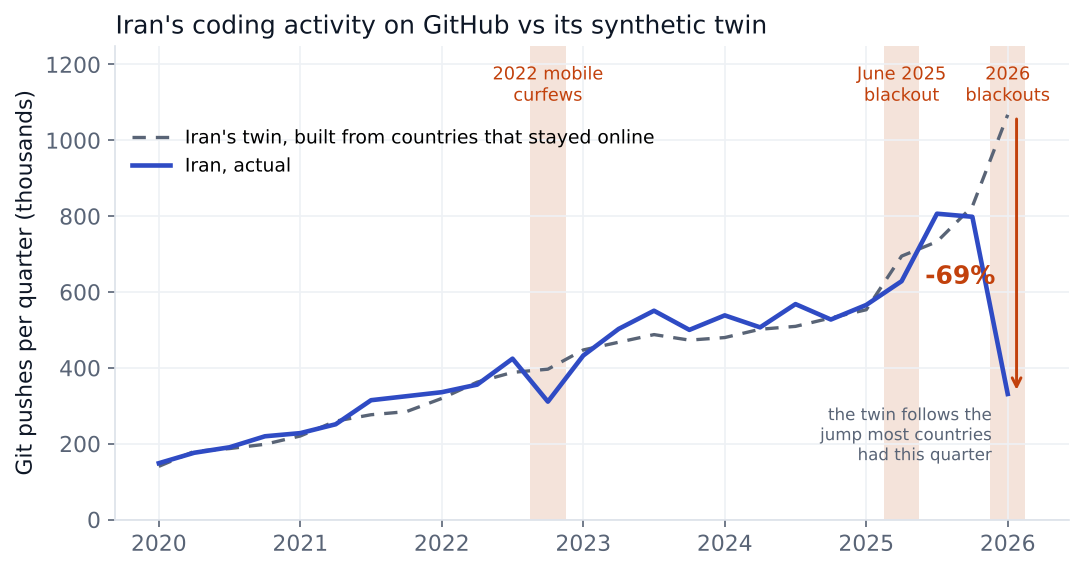
\includegraphics[width=\linewidth]{../figures/iran.png}\\[-3pt]
{\scriptsize\color{mut} The twin is a weighted mix of countries that moved like Iran before the event. The gap after is the effect.}
\end{minipage}

\vspace{4pt}
\textbf{How sure I am}
\begin{itemize}
\item Two methods (synthetic control and synthetic difference in differences) agree within a few points on every clear result, and the results barely move when the donor pool changes.
\item I planted 1,500 fake shutdowns of known size in countries that never had one. False alarms stayed under 3\%, bias within 1.5 points, and a drop of 35\% (about a month offline) was caught 88\% of the time. A drop of 10\% (about 9 days) was caught only 6\% of the time.
\item Every estimate is checked against placebo runs on all 106 control countries and on earlier quarters of the same country.
\end{itemize}

\textbf{What I'd do with this}
\begin{itemize}
\item \textbf{Monitor shutdowns with daily data.} Quarterly country metrics only catch the long ones. Flag known shutdown quarters in any country level forecast instead of treating them as noise.
\item \textbf{Don't forecast a rebound.} Days lost to a shutdown stay lost. The quarter after Iran's 2022 curfews went back to normal, but it didn't make up the gap.
\item \textbf{Use location drift as a cheap early signal.} A fall in accounts placed in a country is a free indicator of VPN use or people leaving, available from data GitHub already publishes.
\item \textbf{Never report a before and after.} With a whole world growing at different speeds, a twin is the minimum for a fair comparison.
\end{itemize}

\textbf{Limits.} Shutdowns come with coups, protests and war, so each number is the cost of the whole crisis. The day by day test is what isolates the internet itself. Iran's twin assumes it would have joined the jump most countries had in early 2026. If it would have stayed flat, the drop is 59\%, which is exactly what its days offline predict.

\end{document}
